\documentclass[border=10pt]{standalone}
\usepackage{tikz}
\usepackage{xcolor}
\usetikzlibrary{shapes.geometric, arrows.meta, positioning, fit, backgrounds, calc}

% Colors
\definecolor{jkcGold}{HTML}{F7931A}
\definecolor{jkcBlue}{HTML}{2E86AB}
\definecolor{jkcGreen}{HTML}{28A745}
\definecolor{jkcRed}{HTML}{DC3545}
\definecolor{darkGray}{HTML}{2D3436}
\definecolor{lightGray}{HTML}{DFE6E9}
\definecolor{orange}{HTML}{FF9F43}
\definecolor{purple}{HTML}{9B59B6}

\begin{document}
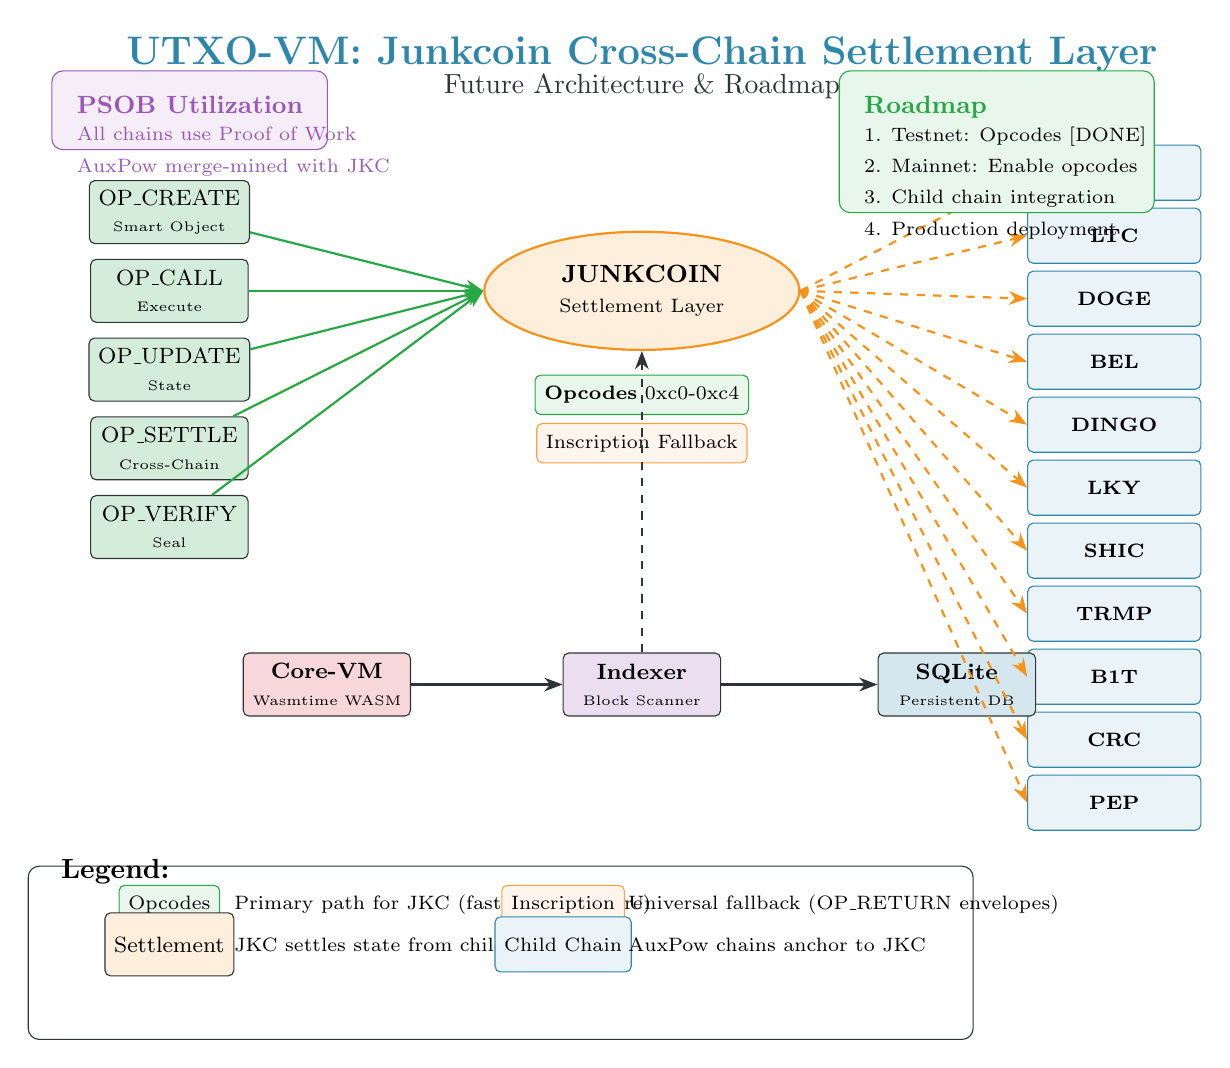
\begin{tikzpicture}[
  node distance=0.8cm,
  every node/.style={font=\small},
  block/.style={rectangle, draw=darkGray, fill=lightGray, minimum width=2cm, minimum height=0.8cm, rounded corners=2pt, align=center, font=\footnotesize},
  chain/.style={rectangle, draw=jkcBlue, fill=jkcBlue!10, minimum width=2.2cm, minimum height=0.7cm, rounded corners=2pt, align=center, font=\scriptsize},
  opcode/.style={rectangle, draw=jkcGreen, fill=jkcGreen!10, minimum width=1.8cm, minimum height=0.5cm, rounded corners=2pt, align=center, font=\scriptsize},
  inscription/.style={rectangle, draw=orange, fill=orange!10, minimum width=1.8cm, minimum height=0.5cm, rounded corners=2pt, align=center, font=\scriptsize},
  settlement/.style={ellipse, draw=jkcGold, fill=jkcGold!15, minimum width=2.5cm, minimum height=0.8cm, align=center, font=\small, thick},
  arrow/.style={-Stealth, thick},
  dashedarrow/.style={-Stealth, thick, dashed},
]

% Title
\node[font=\Large\bfseries, text=jkcBlue] at (8, 9.5) {UTXO-VM: Junkcoin Cross-Chain Settlement Layer};
\node[font=\normalsize, text=darkGray] at (8, 9.1) {Future Architecture \& Roadmap};

% === JUNKCOIN SETTLEMENT LAYER (CENTER) ===
\node[settlement, minimum width=4cm, minimum height=1.5cm] (jkc) at (8, 6.5) {\textbf{JUNKCOIN}\\{\scriptsize Settlement Layer}};

% Opcodes inside JKC
\node[opcode, below=0.3cm of jkc] (opcodes) {\textbf{Opcodes} 0xc0-0xc4};
\node[inscription, below=0.1cm of opcodes] (inscription) {Inscription Fallback};

% === OPCODE PATHS (LEFT) ===
\node[block, fill=jkcGreen!20] (create) at (2, 7.5) {OP\_CREATE\\{\tiny Smart Object}};
\node[block, fill=jkcGreen!20] (call) at (2, 6.5) {OP\_CALL\\{\tiny Execute}};
\node[block, fill=jkcGreen!20] (update) at (2, 5.5) {OP\_UPDATE\\{\tiny State}};
\node[block, fill=jkcGreen!20] (settle) at (2, 4.5) {OP\_SETTLE\\{\tiny Cross-Chain}};
\node[block, fill=jkcGreen!20] (verify) at (2, 3.5) {OP\_VERIFY\\{\tiny Seal}};

% === CHILD CHAINS (RIGHT) ===
\node[chain] (btc) at (14, 8) {\textbf{BTC}};
\node[chain] (ltc) at (14, 7.2) {\textbf{LTC}};
\node[chain] (doge) at (14, 6.4) {\textbf{DOGE}};
\node[chain] (bel) at (14, 5.6) {\textbf{BEL}};
\node[chain] (dingo) at (14, 4.8) {\textbf{DINGO}};
\node[chain] (lky) at (14, 4.0) {\textbf{LKY}};
\node[chain] (shic) at (14, 3.2) {\textbf{SHIC}};
\node[chain] (trmp) at (14, 2.4) {\textbf{TRMP}};
\node[chain] (b1t) at (14, 1.6) {\textbf{B1T}};
\node[chain] (crc) at (14, 0.8) {\textbf{CRC}};
\node[chain] (pep) at (14, 0.0) {\textbf{PEP}};

% === CORE COMPONENTS (BOTTOM) ===
\node[block, fill=jkcRed!20] (vm) at (4, 1.5) {\textbf{Core-VM}\\{\tiny Wasmtime WASM}};
\node[block, fill=purple!20] (indexer) at (8, 1.5) {\textbf{Indexer}\\{\tiny Block Scanner}};
\node[block, fill=jkcBlue!20] (sqlite) at (12, 1.5) {\textbf{SQLite}\\{\tiny Persistent DB}};

% === ARROWS: Opcodes to JKC ===
\draw[arrow, jkcGreen] (create) -- (jkc.west);
\draw[arrow, jkcGreen] (call) -- (jkc.west);
\draw[arrow, jkcGreen] (update) -- (jkc.west);
\draw[arrow, jkcGreen] (settle) -- (jkc.west);
\draw[arrow, jkcGreen] (verify) -- (jkc.west);

% === ARROWS: JKC to Child Chains ===
\draw[dashedarrow, jkcGold] (jkc.east) -- (btc.west);
\draw[dashedarrow, jkcGold] (jkc.east) -- (ltc.west);
\draw[dashedarrow, jkcGold] (jkc.east) -- (doge.west);
\draw[dashedarrow, jkcGold] (jkc.east) -- (bel.west);
\draw[dashedarrow, jkcGold] (jkc.east) -- (dingo.west);
\draw[dashedarrow, jkcGold] (jkc.east) -- (lky.west);
\draw[dashedarrow, jkcGold] (jkc.east) -- (shic.west);
\draw[dashedarrow, jkcGold] (jkc.east) -- (trmp.west);
\draw[dashedarrow, jkcGold] (jkc.east) -- (b1t.west);
\draw[dashedarrow, jkcGold] (jkc.east) -- (crc.west);
\draw[dashedarrow, jkcGold] (jkc.east) -- (pep.west);

% === ARROWS: Core Components ===
\draw[arrow, darkGray] (vm) -- (indexer);
\draw[arrow, darkGray] (indexer) -- (sqlite);
\draw[dashedarrow, darkGray] (indexer.north) -- (jkc.south);

% === LEGEND ===
\node[draw=darkGray, fill=white, rounded corners, minimum width=12cm, minimum height=2.2cm, anchor=north west] at (0.2, -0.8) {};
\node[font=\bfseries, anchor=north west] at (0.5, -0.6) {Legend:};

\node[opcode, minimum width=1.2cm] at (2, -1.3) {Opcodes};
\node[font=\scriptsize, anchor=west] at (2.7, -1.3) {Primary path for JKC (fast, cheap, secure)};

\node[inscription, minimum width=1.2cm] at (7, -1.3) {Inscription};
\node[font=\scriptsize, anchor=west] at (7.7, -1.3) {Universal fallback (OP\_RETURN envelopes)};

\node[block, minimum width=1.2cm, fill=jkcGold!15] at (2, -1.8) {Settlement};
\node[font=\scriptsize, anchor=west] at (2.7, -1.8) {JKC settles state from child chains};

\node[chain, minimum width=1.2cm] at (7, -1.8) {Child Chain};
\node[font=\scriptsize, anchor=west] at (7.7, -1.8) {AuxPow chains anchor to JKC};

% === ROADMAP (TOP RIGHT) ===
\node[draw=jkcGreen, fill=jkcGreen!10, rounded corners, minimum width=4cm, minimum height=1.8cm, anchor=north west] at (10.5, 9.3) {};
\node[font=\bfseries\small, anchor=north west, text=jkcGreen] at (10.7, 9.1) {Roadmap};
\node[font=\scriptsize, anchor=north west] at (10.7, 8.7) {1. Testnet: Opcodes [DONE]};
\node[font=\scriptsize, anchor=north west] at (10.7, 8.3) {2. Mainnet: Enable opcodes};
\node[font=\scriptsize, anchor=north west] at (10.7, 7.9) {3. Child chain integration};
\node[font=\scriptsize, anchor=north west] at (10.7, 7.5) {4. Production deployment};

% === PSOB NOTE ===
\node[draw=purple, fill=purple!10, rounded corners, minimum width=3.5cm, minimum height=1cm, anchor=north west] at (0.5, 9.3) {};
\node[font=\bfseries\small, anchor=north west, text=purple] at (0.7, 9.1) {PSOB Utilization};
\node[font=\scriptsize, anchor=north west, text=purple] at (0.7, 8.7) {All chains use Proof of Work};
\node[font=\scriptsize, anchor=north west, text=purple] at (0.7, 8.3) {AuxPow merge-mined with JKC};

\end{tikzpicture}
\end{document}
